\chapter{Geschichtliche Übersicht}
\label{ch:Geschichtlich}

In der Geschichte von Hypertext sind viele verschiedene Konzepte und Systeme entstanden. In diesem Kapitel werden für einen Überblick einige davon vorgestellt. Das Konzept hinter Hypertext kann auf einen Artikel aus dem Jahr 1945 zurückgeführt werden.

\begin{quote}
	\glqq Consider a future device for individual use, which is a sort of mechanized private file and library. It needs a name, and to coin one at random, memex will do. A memex is a device in which an individual stores all his books, records, and communications, and which is mechanized so that it may be consulted with exceeding speed and flexibility.\grqq{ }\cite[Section 6]{Bush1945}.
\end{quote}

Im Jahr 1945 wurde \glqq As we may think\grqq{ }von Vannevar Bush veröffentlicht. Mit dem Konzept \glqq Memex\grqq{ } erdachte Vannevar Bush eine Maschine für die individuellen Verwendung - eine private, mechanisierte Bibliothek. Die \ref{fig:memex} zeigt eine Illustration aus dem Life Magazine 1945. Wenn der Nutzer ein bestimmtes Buch aufrufen möchte, könne er einen Code in das Keyboard eintippen und die Titelseite erscheint als Projektion \cite[S.121]{Life1945} \cite[Section 6]{Bush1945}. In in diesem Konzept könne der Nutzer einen sogenannten \glqq main trail\grqq{ }aus Dokumenten erstellen. Dieser Trail solle eine Kombination aus Dokumenten sein, die aus der Perspektive des Nutzers von Interesse ist. Mit sogenannten \glqq side tails\grqq{ }könne der Nutzer ein Main Trail mit anderen Dokumenten \glqq verlinkt\grqq{ }\cite[Section 7]{Bush1945}. Diese Trails könnten als erstes Konzept von Hyperlinks verstanden werden. Zwei Jahrzehnte nach der Veröffentlichung von \glqq As we may think\grqq{ }, in der 1960er Jahren, wurde der erst der Begriff Hypertext von Ted Nelson geprägt. 

\begin{figure}[!ht]
	\centering
	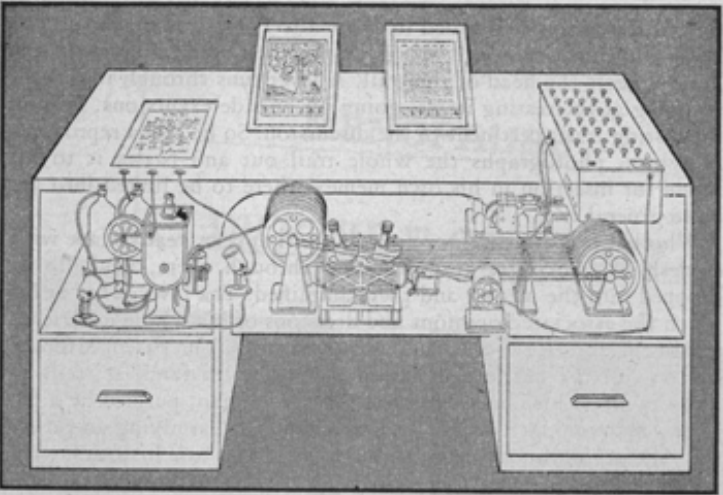
\includegraphics[width=0.6\textwidth]{image/memex}
	\caption{\glqq Memex in the form of a desk would instantly bring files and material on any subject to the operator's fingertips. [...] At left is a mechanism which automatically photographs longhead notes, pictures and letters, then files them in the desk for future reference\grqq{ } \cite[S.123]{Life1945}}
	\label{fig:memex}
\end{figure}

\begin{quote}
	\glqq Let me introduce the word hypertext to mean a body of written or pictorial material interconnected in such a complex way that it could not conveniently be presented or represented on paper. It may contain summaries, or maps of its contents and theier interrelations; it may contain annotations, additions and footnotes from scholars who have examined it. [...]\grqq{ }\cite{Nelson1965}
\end{quote}

Nach Ted Nelson habe ein System auf Papier gravierende Einschränkungen beim Organisieren oder Präsentieren von Ideen. Ein Buch würde nie perfekt zu einem Leser passen. Der eine Leser sei gelangweilt, während ein anderer von den gleichen Seiten verwirrt werde. \glqq Ein solches System könne das Potenzial haben, das Gefühl der Freiheit, die Motivation und das intellektuelle Verständnis des Lesenden zu vergrößern\grqq{ }\cite{Nelson1965}. 

\begin{section}{NLS und AUGMENT}
\label{sec:nls}

Im gleichen Jahrzehnt erschien Doug Engelbarts \glqq Augmenting Human Intellect: A Conceptual Framework\grqq{ }. 

\begin{quote}
\glqq By augmenting human intellect we mean increasing the capability of a man to approach a complex problem situation [...].\grqq{ }\cite[S. 1]{Engelbart1962}
\end{quote}

Engelbart schrieb in \glqq Augmenting Human Intellect: A Conceptual Framework\grqq{ } von dem \glqq digital computer as a tool for the personal use of an individual. Here there is not only promise of great flexibility in the composing and rearranging of text [...]\grqq{ }\cite[S. 17]{Engelbart1962}. Während seiner Arbeit am Augmentation Research Center am Stanford Research Institute (SRI-ARC) wurde unter anderem das \glqq NLS\grqq{ }(the oN-Line System) entwickelt. Wobei \glqq on-line\grqq{ }in den 60er Jahren nicht die gleiche Bedeutung gehabt haben dürfte als Heute. Vorgestellt wurde das NLS auf der Fall Joint Computer Conference in San Francisco 1968. Diese Präsentation wird oft \glqq mother of all demos\grqq{ }genannt. Neben dem NLS wurden auch die interaktive Textverarbeitung, die Computermaus und die Organisation von Windows auf dem Bildschirm (Siehe \ref{fig:mother}). Das NLS würde präsentiert als \glqq ein mächtiges Tool für die Arbeit eines Individuums, wenn er studiert, plant, designt, debuggt oder dokumentieren.\grqq{ }\cite{MotherOfDemo1968}. Es gäbe Möglichkeiten für das kollaborative Arbeiten, es gäbe gemeinsame Dokumente und man könne Nachrichten an Dokumente heften \cite{MotherOfDemo1968}. 

\begin{figure}[!ht]
	\centering
	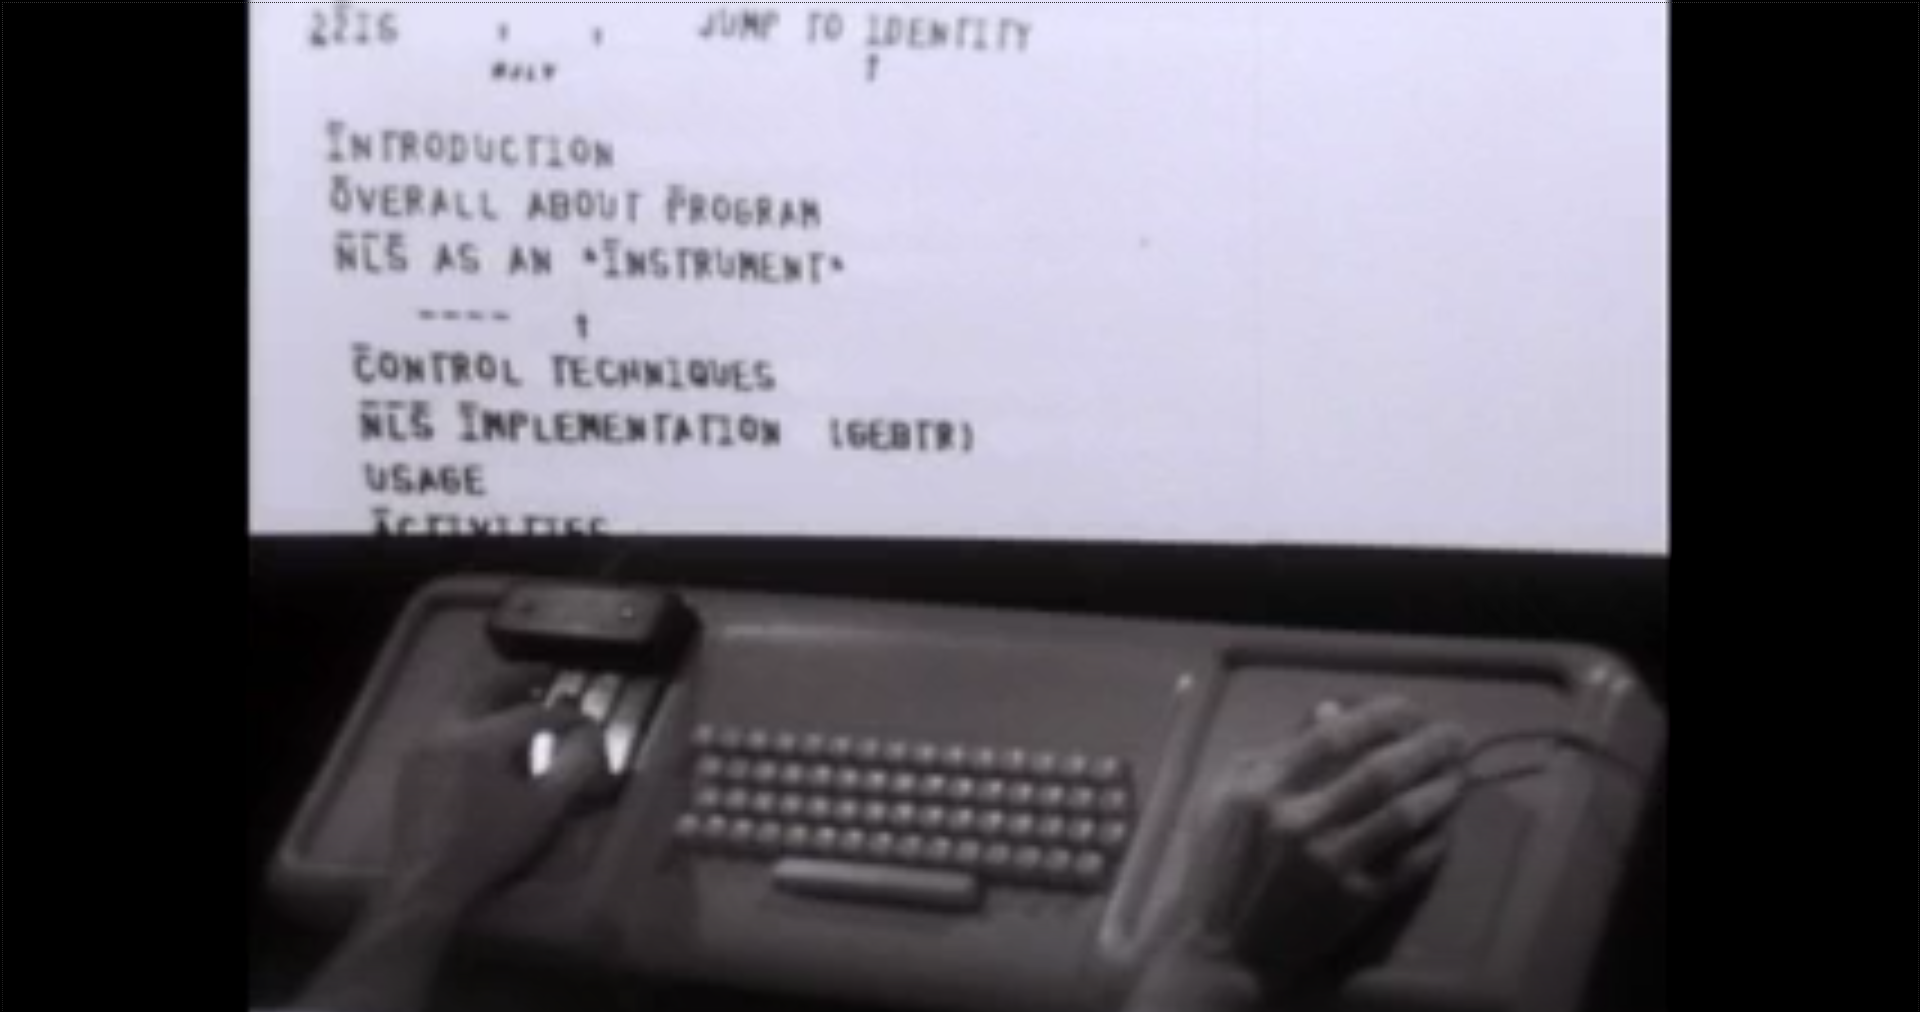
\includegraphics[width=0.8\textwidth]{image/mother}
	\caption{Doug Engelbart präsentiert auf der Fall Joint Computer Conference in San Francisco die Forschung vom Stanford Research Institute \cite{MotherOfDemo1968}.}
	\label{fig:mother}
\end{figure}

Gezeigt wurden aber auch die Hypertext Funktionalitäten, Dokumente seien verknüpft mit Links und der Nutzer könne entscheiden welchen \glqq Branch\grqq{ }er betrete \cite{MotherOfDemo1968}. Verlinkungen konnten durch verschiedene Adressiermöglichkeiten realisiert werden. Jedes Dokument in NLS ist in \glqq Statements\grqq{ }unterteilt und diese Statements konnten auf verschiedene Weisen verlinkt werden \cite{Engelbart1984}. Jedes Statement hat eine \glqq structural statement number\grqq{ }, eine eindeutige ID, die sind nach der Position in einem Dokument richtet. Nach dem Verändern des Textes konnten so Links zu falschen Statements führen. Der \glqq statement identifiers\grqq{ }, als globale ID war unabhängig von der Position des Statements, diese ID blieb unverändert und \glqq Labels\grqq{ }die vom Nutzer definiert werden. Das Userinterface bot Kommandos zum Manipulieren der Oberfläche. Es konnten Outlines und eine Art Vorschau der ersten Zeilen von jedem Statement angezeigt werden. Die Verlinkungen und Bedienmöglichkeiten ermöglichten dem Nutzer ein \glqq herein und heraus zoomen \grqq{ }\cite{MotherOfDemo1968}. Die kommerziellen Rechte an dem System wurden 1978 an Tymshare abgegeben und NLS wurde zu AUGMENT umbenannt \cite{Engelbart1984}. Im Vergleich zum Konzept Memex hatte das Team um das NLS ähnliche Ziele. Die Arbeit des Individuums sollte optimiert werden. Die Memex als analoges Konzept und das NLS als digitale Lösung für ein Hypertext-System. Die Verknüpfungen der Dokumente in der Memex Maschine sind vergleichbar mit den verlinkten Statements im NLS, beide Verlinkungen wurden auch über IDs realisiert \cite{Engelbart1984}, \cite{Bush1945}. Nur die Nutzereingabe unterscheidet sich bei beiden, staa Touch und Spracheingabe \cite{Bush1945} nutzte das Team rund um Doug Engelbart Maus und Tastatur \cite{MotherOfDemo1968}.

\end{section}

\begin{section}{Problem: Dangling edges}
\label{sec:dangling}

Allerdings wäre Vannevar Bush bei einer Realisierung der Memex wahrscheinlich auf das gleiche Problem gestoßen wie Doug Engelbart. Ein Hypertext ist vergleichbar mit einem Graphen aus Nodes und Edges. Ein Text könnte ein Node sein und eine Verlinkungen zwischen zwei Texten ist eine Edge zwischen zwei Nodes. Durch entfernen von Nodes können \glqq dangling edges\grqq{ }entstehen. Die \ref{fig:dangle} zeigt zum Beispiel durch das Entfernen des Textes $D$ zwei entstandenen Dangling Edges von $A$ und $E$. Bei NLS konnte durch das Bearbeiten der Dokumente oder Statements Dangling Edges entstehen. Dies könnte durch die verschiedenen Adressiermöglichkeiten zumindest eingedämmt werden \cite{Engelbart1984}.

\begin{figure}[!ht]
	\centering
	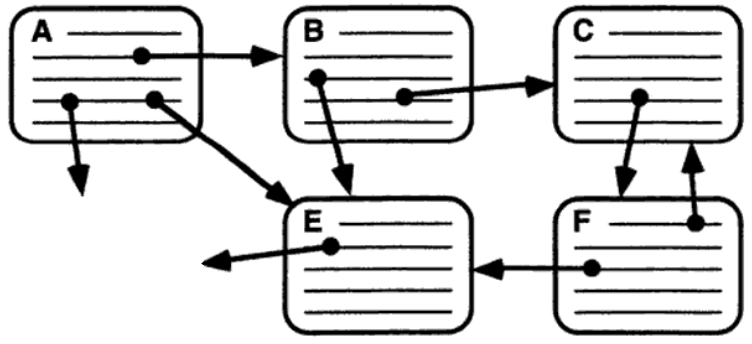
\includegraphics[width=0.8\textwidth]{image/dangle}
	\caption{Modifizierte Darstellung von Nielsen, zur Darstellung von Dangling Edges \cite[S.1]{Nielsen1995}.}
	\label{fig:dangle}
\end{figure}

\end{section}





